\chapter{Results}
\section{System}
During the building process it became more and more clear that this project would be more of a \gls{Proof of Concept} other than a fully fetched, commercially viable product. There are just too many factors and variables that need to be considered in building a long-lasting, reliable, off-the-grid, weatherproof, accurate measuring system. For this reason, the system was more of a proof of concept than an \gls{Off the shelf} product and still needs some improvements to be made before it can be used in a real-world scenario.

Nonetheless, the resulting system fulfilled most of the requirements outlined in the planning phase and provides a solid base to be improved upon in the future. It fulfills its core functionality goals of collecting measurements of a beehive in a remote location and transmitting them to a central server where it can be accessed by a user interface. 

\begin{figure}
    \centering
    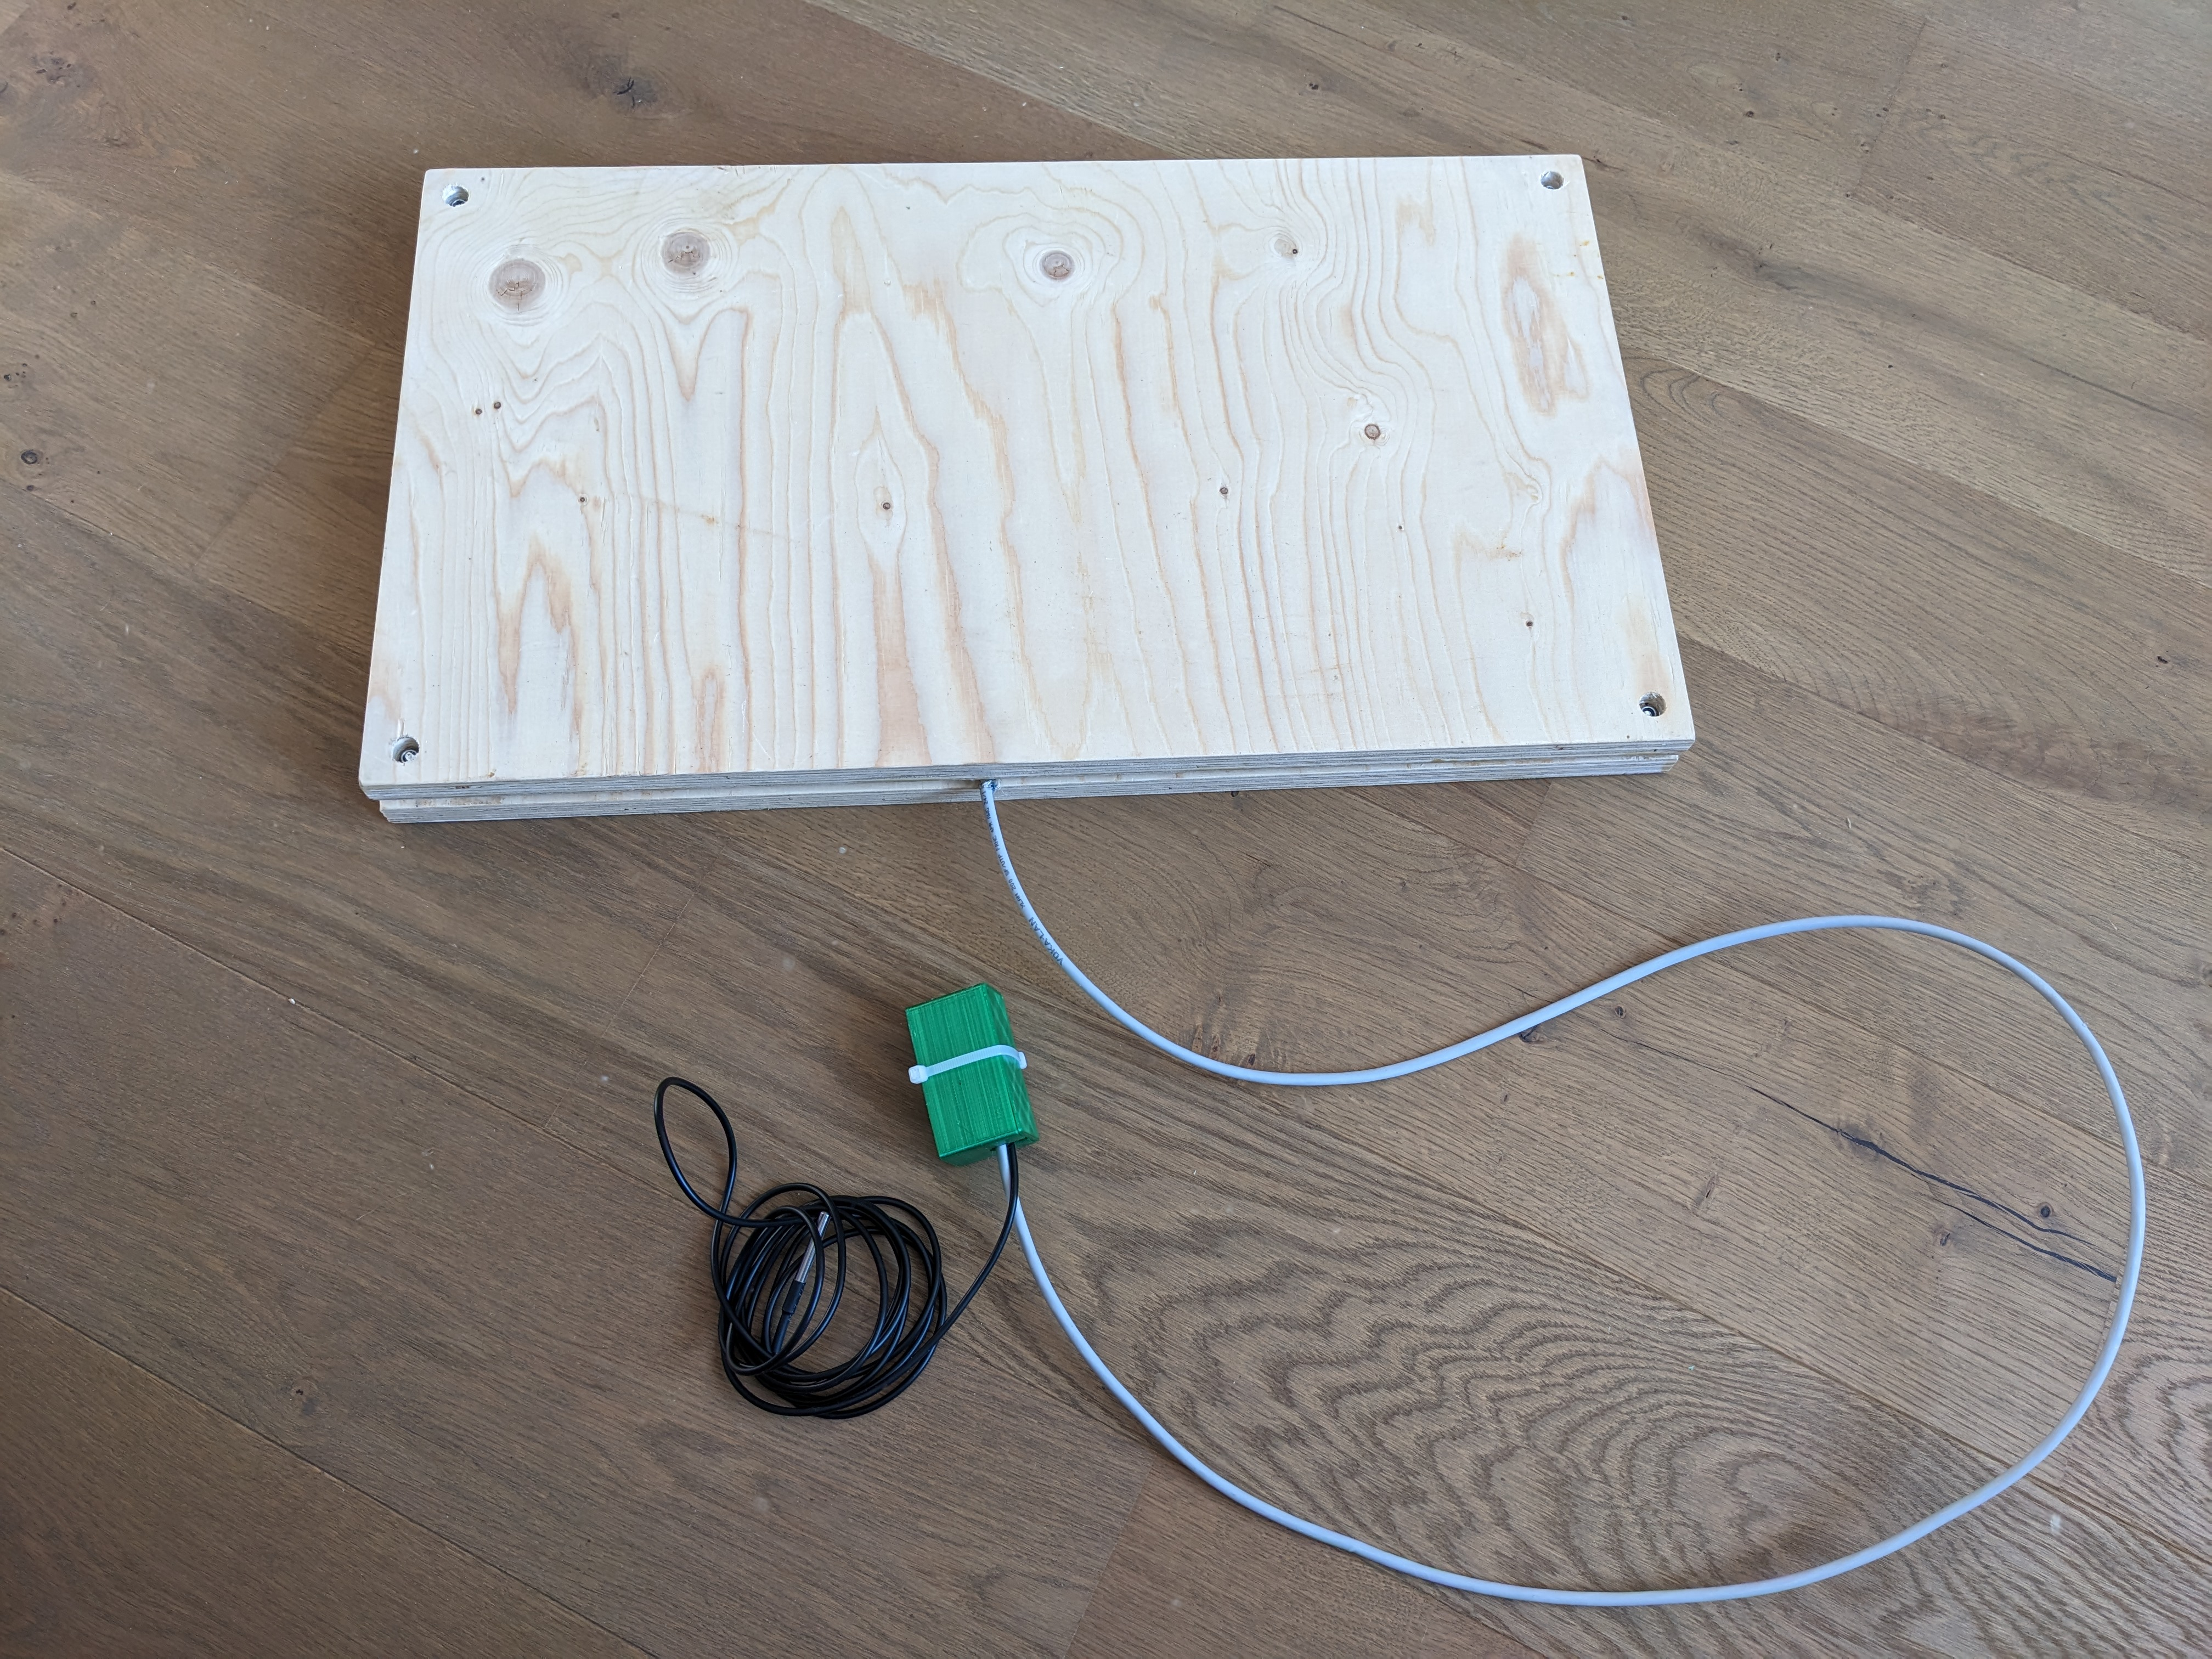
\includegraphics[width=0.55\textwidth]{figures/scale.jpg}
    \caption{Overview of the system}
    \label{fig:overview}
\end{figure}

\begin{figure}
    \centering
    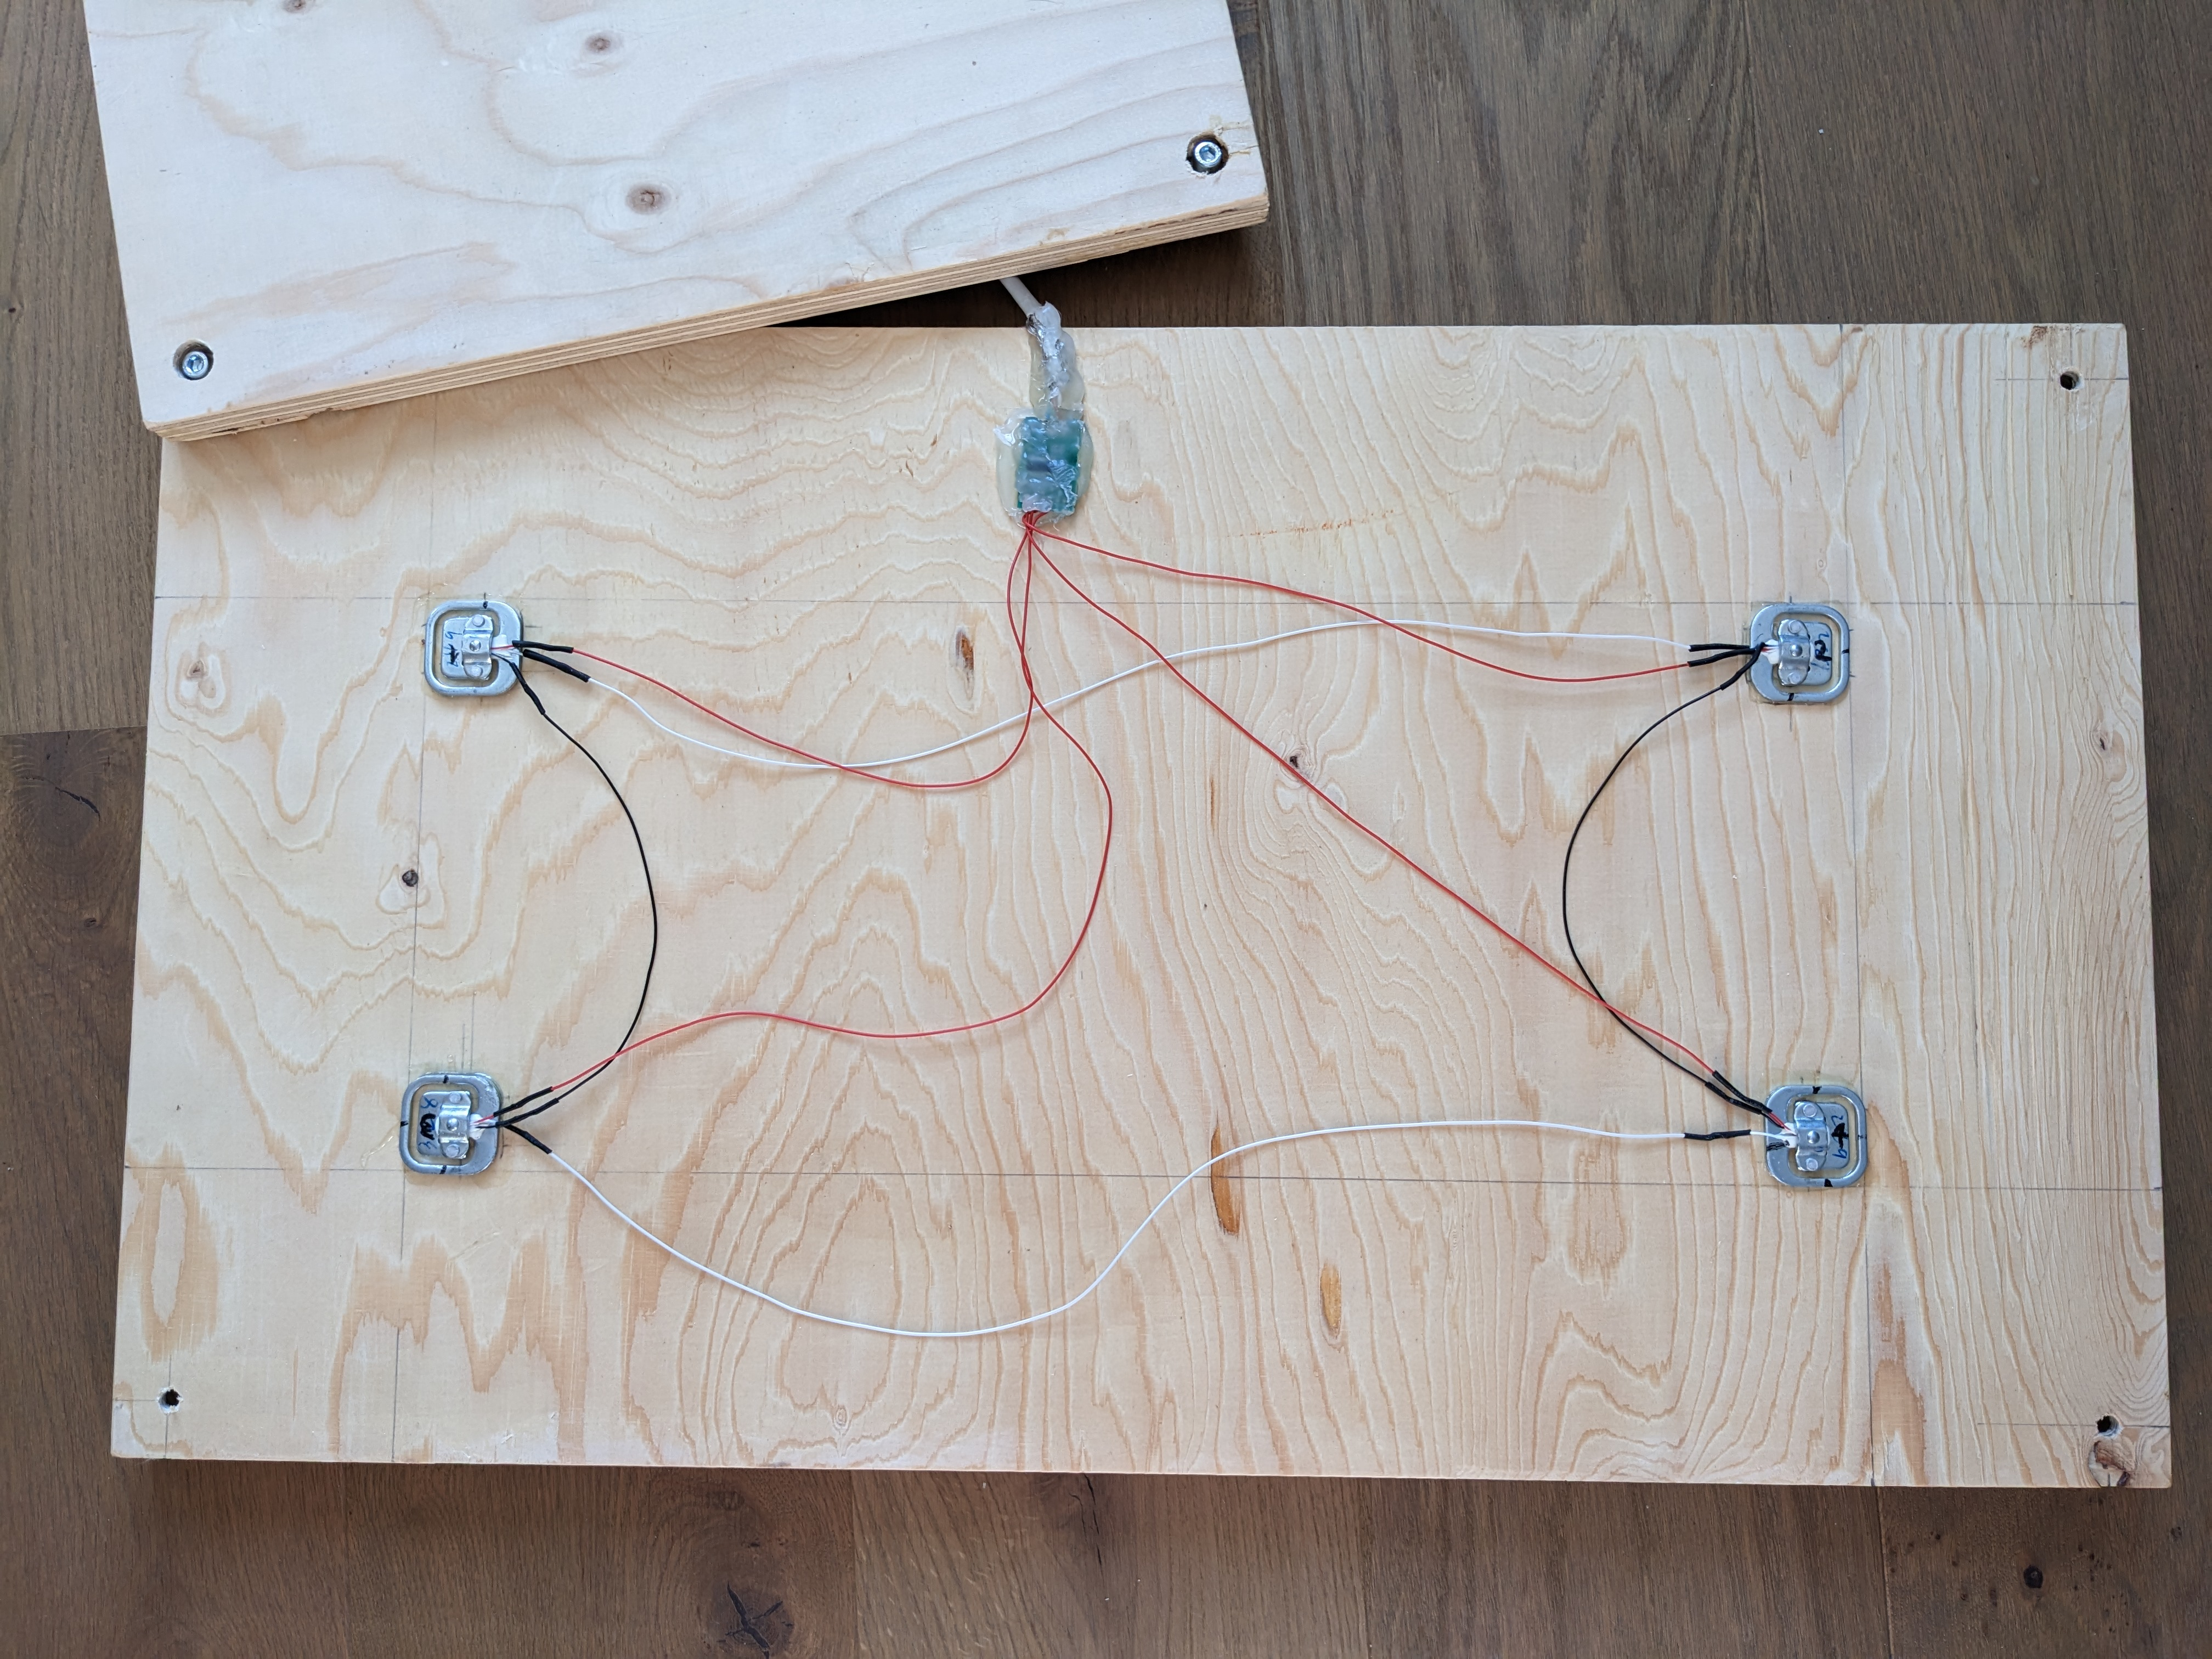
\includegraphics[width=0.55\textwidth]{figures/scale_wiring.jpg}
    \caption{Internal wiring of the scale}
    \label{fig:overview}
\end{figure}

\begin{figure}
    \centering
    \includegraphics[width=0.55\textwidth]{figures/esp32_connected.jpg}
    \caption{Internal wiring of the microcontroller}
    \label{fig:overview}
\end{figure}

\newpage
\newpage
\section{Costs}
The main goal of this project was to make the system as cost-effective as possible. The following table shows the total cost it took to build the system.

\begin{table}[ht]
    \centering
    \begin{bfhTabular}{llll}
       Name & Quantity & Price & Total
       \\\hline
       Wood & \num{1} & CHF\num{41.00} & CHF\num{41.00}\\\hline
       Wood Treatment & \num{1} & CHF\num{3.00} & CHF\num{3.00}\\\hline
       Cables & \num{1} & CHF\num{3.00} & CHF\num{3.00}\\\hline
       Temperature Sensor (DS18B20) & \num{1} & CHF\num{10.90} & CHF\num{10.90}\\\hline
       18650 LiPo Battery & \num{4} & CHF\num{8.90} & CHF\num{35.60}\\\hline
       LiPo Battery 4x Shield & \num{1} & CHF\num{16.90} & CHF\num{16.90}\\\hline
       Generic Load Cell & \num{4} & CHF\num{4.50} & CHF\num{18.00}\\\hline
       HX711 Load Cell Amplifier & \num{1} & CHF\num{4.50} & CHF\num{4.50}\\\hline
       LILYGO TTGO T-Call ESP32 SIM800L & \num{1} & CHF\num{25.17} & CHF\num{25.17}\\\hline
       Misc. Nuts, Bolts and other consumables & \num{1} & CHF\num{10.00} & CHF\num{10.00}\\\hline
       Data Plan for 365 Days & \num{1} & CHF\num{44.00} & CHF\num{44.00}\\\hline
        &  & \textbf{Total} & \textbf{CHF212.07}\\\hline
    \end{bfhTabular}
    \caption{Price of the system}
    \label{tab:tab1}
 \end{table}

This is way cheaper than even the cheaper commercially available beehive monitoring systems with the added benefit of being completely open source and customizable. This price doesn't include the time it took to build the system, which is a significant factor in the total cost of the system. Most of the time however was spent on the design, planning and research phase, which wouldn't need to be done again  for future iterations of the system.

 \newpage
\section{Conclusion}
\subsection{Future Improvements}
The system as it is right now is not really usable in the way it was intended. There are still some major improvements that need to be done like changing the material of the scale to something less subjectable to thermal expansion and addressing the load cell inaccuracies. Another important aspect is creating a weatherproof housing for the microcontroller and the batteries.

Another important aspect is providing solar power to the batteries. This would reduce the need for frequent battery changes and would make the system more reliable.

More user interfaces like SMS/Email notifications would also be a nice addition to the system.

Another interesting future prospect would be the addition of data analysis to the system. This would allow the user to get a better understanding of the data collected by the system and would allow for better decision-making. There could also be systems to make predictions about the future based on the data collected. For example a prediction of when the honey will be ready to harvest and how much the expected yield will be. Another system would be the prediction and detection of a swarm. This would allow the user to take action before the swarm leaves the hive and would allow for better swarm management.

\newpage
\subsection{Reflection}
All in all I think this project was a success. I was able to come up with a setup that did what it was supposed to do. Furthermore, I have learned a lot about designing and building IOT projects and the technologies used in the project. I am looking forward to improving the system in the future and transforming it into a completely viable product. It is also my intention to make the system open source and share it with the community.

During the project, I encountered some quite significant roadblocks, that I was able to overcome. I believe that this greatly improved my problem-solving skills and my ability to work under pressure. A lot of the problems I encountered were in fields I had no experiences in, which made it even more challenging. But I believe that solving those issues and thinking about the problems that arose made me a better engineer.

In conclusion, I really enjoyed working on this project, and I am looking forward to start working on my bachelor thesis.
